%% The following is a directive for TeXShop to indicate the main file
%%!TEX root = diss.tex

\chapter{Algorithms for Thue-Mahler Equations}
\label{ch:AlgorithmsForTM}

\begin{enumerate}
\item First Steps \autoref{sec:FirstSteps}
\item rel number field \autoref{sec:RelevantAlgNumField}
\item Lattices \autoref{sec:Lattices}
\item Setup with Lemmata from Samir
\item LLL [DONE - roughly]
\item Fincke-Pohst with changes from Benjamin [DONE- roughly]
\item linear forms in logs
\end{enumerate}

%--------------------------------------------------------------------------------------------------------------------------------------------%
%--------------------------------------------------------------------------------------------------------------------------------------------%

\section{First steps}
\label{sec:FirstSteps}

Fix a nonzero integer $c$ and let $S=\{p_1,\dotsc,p_v\}$ be a set of rational primes. Let
\[F(X,Y) = c_0 X^n + c_1 X^{n-1}Y + \cdots + c_{n-1}XY^{n-1} + c_nY^n\]
be an irreducible binary form over $\mathbb{Z}$ of degree $n \geq 3$. We want to solve the Thue--Mahler equation
\begin{equation} \label{eq:ThueMahler}
F(X,Y) = c p_1^{Z_1}\cdots p_v^{Z_v}
\end{equation}
for unknowns $X,Y, Z_1, \dots, Z_v$ with $\gcd(X,Y) = 1$ and $Z_i \geq 0$ for $i = 1,\dots, v$. To do so, we first reduce \eqref{eq:ThueMahler} to the special case where $c_0 = 1$ and $\gcd(c,p_i) = 1$ for $i = 1, \dots, v$. 

As $F$ is irreducible by assumption, at least one of the coefficients $c_0$ and $c_n$ is nonzero. Hence, we may transform the given Thue--Mahler equation to one with $c_0 \neq 0$ by interchanging $X$ and $Y$ and by renaming the coefficients $c_i$ appropriately. In particular, solving \eqref{eq:ThueMahler} is equivalent to solving 
\[ c_0' \overline{X}^n + c_1' \overline{X}^{n-1}\overline{Y} + \cdots + c_{n-1}'\overline{X}\overline{Y}^{n-1} + c_n'\overline{Y}^n = c p_1^{Z_1}\cdots p_v^{Z_v},\]
where $c_i' = c_{n-1}$ for $i = 0, \dots, n$, $\overline{X} = Y$, and $\overline{Y} = X$. 

Denote by $\mathcal{D}$ the set of all positive rational integers $m$ dividing $c_0$ such that ${\ord_p(m)\leq \ord_p(c)}$ for each rational prime $p\notin S$. Equivalently, $\mathcal{D}$ is precisely the set of all possible integers $d$ such that $d = \gcd(c_0,Y)$. To see this, let $q_1, \dots, q_{w}$ denote the distinct prime divisors of $a$ not contained in $S$. Then 
\[c = \prod_{i=1}^w q_i^{b_i}\cdot \prod_{i=1}^v p_i^{\ord_{p_i}(c)}\]
for some integers $b_i >0$. If $(X,Y,Z_1, \dots, Z_v)$ is a solution of the Thue-Mahler equation in question, it follows that
\[F(X,Y) = cp_1^{Z_1}\dots p_v^{Z_v} =  \prod_{i=1}^w q_i^{b_i}\cdot \prod_{i=1}^v p_i^{\ord_{p_i}(c) + Z_i}.\]
Suppose $\gcd(c_0,Y) = d$. Since $d$ divides $F(X,Y)$, it necessarily divides 
\[{\prod_{i=1}^w q_i^{b_i}\cdot \prod_{i=1}^v p_i^{\ord_{p_i}(c) + Z_i}}.\] 
In particular, 
\[d = \prod_{i=1}^w q_i^{s_i}\cdot \prod_{i=1}^v p_i^{t_i}\]
for some non-negative integers $s_1, \dots, s_w, t_1, \dots, t_v$ such that 
\[s_i \leq \min\{\ord_{q_i}(c), \ord_{q_i}(c_0)\} \quad \text{ and } \quad 
	t_i \leq \min\{\ord_{p_i}(c) + Z_i, \ord_{p_i}(c_0)\}.\] 
From here, it is easy to see that ${\ord_p(d)\leq \ord_p(c)}$ for each rational prime $p\notin S$ so that $d \in \mathcal{D}$. 

Conversely, suppose $d \in \mathcal{D}$ so that $\ord_{p}(d) \leq \ord_{p}(c)$ for all $p \notin S$. That is, the right-hand side of 
\[\ord_{p}(d) \leq \ord_{p}(c) = 
\ord_p\left(\prod_{i=1}^w q_i^{b_i}\cdot \prod_{i=1}^v p_i^{\ord_{p_i}(c)}\right)\]
is non-trivial only at the primes $\{q_1, \dots, q_w\}$. In particular, 
\[d = \prod_{i=1}^w q_i^{s_i}\cdot \prod_{i=1}^v p_i^{t_i}\]
for non-negative integers $s_1, \dots, s_w, t_1, \dots, t_v$ such that 
\[s_i \leq \min\{\ord_{q_i}(c), \ord_{q_i}(c_0)\} \quad \text{ and } \quad 
	t_i \leq \ord_{p_i}(c_0).\] 
It follows that $d = \gcd(c_0,Y)$ for some solution $(X,Y,Z_1, \dots, Z_v)$ of equation~\eqref{eq:ThueMahler}. 

For any $d\in \mathcal{D}$, we define the rational numbers 
\[u_d = c_0^{n-1}/d^n \quad \textnormal{and}\quad c_d = \sgn(u_dc)\prod_{p\notin S} p^{\ord_p(u_dc)}.\]
On using that $d\in \mathcal{D}$, we see that the rational number $c_d$ is in fact an integer coprime to $S$. 

Suppose $(X,Y,Z_1, \dots, Z_v)$ is a solution of \eqref{eq:ThueMahler} with ${\gcd(X,Y) = 1}$ and $d = \gcd(c_0,Y)$. Define the homogeneous polynomial $f(x,y) \in \mathbb{Z}[x,y]$ of degree $n$ by
\[f(x,y) = x^n + C_1 x^{n-1}y + \dots + C_{n-1}xy^{n-1} + C_ny^n,\]
where
\[x=\tfrac{c_0X}{d},\quad y=\tfrac{Y}{d} \quad \text{ and } \quad C_i = c_ic_0^{i-1} \quad \text{ for } i = 1, \dots, n.\]
Since $\gcd(X,Y) = 1$, the numbers $x$ and $y$ are also coprime integers by definition of $d$. We observe that 
\[f(x,y) = u_dF(X,Y) = u_dc \prod_{i = 1}^v p_i^{Z_i} = c_d\prod_{p \in S}p^{Z_i + \ord_p(u_dc)}.\]
Setting $z_i = Z_i + \ord_p(u_dc)$ for all $i \in \{1, \dots, v\}$, we obtain
\begin{equation} \label{eq:ThueMahler2}
f(x,y) = x^n + C_1 x^{n-1}y + \dots + C_{n-1}xy^{n-1} + C_ny^n = c_d p_1^{z_1}\cdots p_v^{z_v}, 
\end{equation}
where $\gcd(x,y) = 1$ and $\gcd(c_d,p_i) = 1$ for all $i = 1, \dots, v$. 

Since there are only finitely many choices for $d = \gcd(c_0, Y)$, there are only finitely many choices for $\{c_d,u_d,d\}$. Then, solving \eqref{eq:ThueMahler} is equivalent to solving the finitely many Thue-Mahler equations \eqref{eq:ThueMahler2} for each choice of $\{c_d,u_d,d\}$.  For each such choice, the solution $\{x,y,z_1, \dots, z_v\}$ is related to $\{X,Y, Z_1, \dots, Z_v\}$ via
\[X = \frac{dx}{c_0},\quad Y=dy \quad \text{ and } \quad Z_i = z_i - \ord_p(u_dc).\]

Lastly, we observe that the polynomial $f(x,y)$ of \eqref{eq:ThueMahler2} remains the same for any choice of $\{c_d,u_d,d\}$. Thus, to solve the family of equations \eqref{eq:ThueMahler2}, we need only to enumerate over every possible $c_d$. Now, if $\mathcal{C}$ denotes the set of all $\{c_d,u_d,d\}$ and $d_1, d_2 \in \mathcal{D}$, we may have $\{c_{d_1},u_{d_1}, d_1\}, \{c_{d_2},u_{d_2}, d_2\} \in \mathcal{C}$ where $c_{d_1} = c_{d_2}$. That is, $d_1, d_2$ may yield the same value of $c_d$, reiterating that we need only solve \eqref{eq:ThueMahler2} for each distinct $c_d$. 

%--------------------------------------------------------------------------------------------------------------------------------------------%
%--------------------------------------------------------------------------------------------------------------------------------------------%

\section{The relevant algebraic number field}
\label{sec:RelevantAlgNumField}

For the remainder of this chapter, we consider the Thue-Mahler equation
\begin{equation} \label{eq:ThueMahler3}
f(x,y) = x^n + C_1 x^{n-1}y + \dots + C_{n-1}xy^{n-1} + C_ny^n = c p_1^{z_1} \cdots p_v^{z_v}
\end{equation}
where $\gcd(x,y) = 1$ and $\gcd(c,p_i) = 1$ for $i = 1, \dots, p_v$.

Following \edit{Tzanakis, de Weger, Hambrook}, put
\[g(t) = f(t,1) = t^n + C_1 t^{n-1} + \dots + C_{n-1}t + C_n\]
and note that $g(t)$ is irreducible in $\mathbb{Z}[t]$. Let $K = \mathbb{Q}(\theta)$ with $g(\theta) = 0$. Now \eqref{eq:ThueMahler3} is equivalent to the norm equation
\begin{equation} \label{eq:normTM}
N_{K/\mathbb{Q}}(x-y\theta) = cp_1^{z_1}\dots p_v^{z_v}.
\end{equation}

Let $p_i$ be any rational prime and let 
\[(p_i)\mathcal{O}_K = \prod_{j = 1}^{m_i} \mathfrak{p}_{ij}^{e(\mathfrak{p}_{ij}|p_i)}\]
be the factorization of $p_i$ into prime ideals in the ring of integers $\mathcal{O}_K$ of $K$. Let $f(\mathfrak{p}_{ij}|p_i)$ be the inertial degree of $\mathfrak{p}_{ij}$ over $p_i$. Since $N(\mathfrak{p}_{ij}) = p_i^{f_{ij}}$, \eqref{eq:normTM} leads to finitely many ideal equations of the form
\begin{equation} \label{eq:idealTM}
(x-y\theta)\mathcal{O}_K = \mathfrak{a} \prod_{j = 1}^{m_1} \mathfrak{p}_{1j}^{z_{1j}} \cdots \prod_{j = 1}^{m_v} \mathfrak{p}_{vj}^{z_{vj}}
\end{equation}
where $\mathfrak{a}$ is an ideal of norm $|c|$ and the $z_{ij}$ are unknown integers related to $z_i$ by 
\[\sum_{j = 1}^{m_i} f(\mathfrak{p}_{ij}|p_i)z_{ij} = z_i\]
for $i \in \{1, \dots, v\}$.

Our first task is to cut down the number of variables appearing in \eqref{eq:idealTM}. We will do this by showing that only a few prime ideals can divide $(x-y\theta)\mathcal{O}_K$ to a large power. 

%--------------------------------------------------------------------------------------------------------------------------------------------%
%--------------------------------------------------------------------------------------------------------------------------------------------%

\section{The prime ideal removing lemma}
\label{sec:PIRL}

In this section, we establish some key results that will allow us to cut down the number of prime ideals that can appear to a large power in the factorization of $(x-y\theta)\mathcal{O}_K$. It is of particular importance to note that we do not appeal to the Prime Ideal Removing Lemma of Tzanakis, de Weger \edit{ref and Hambrook} here and instead apply the following results of \edit{cite new paper}

Let $p \in \{p_1, \dots, p_v\}$. We will produce the following two finite lists $L_p$ and $M_p$. The list $L_p$ will
consist of certain ideals $\mathfrak{b}$ of $\mathcal{O}_K$ supported at the prime ideals above $p$. The list $M_p$ will consist of certain pairs $(\mathfrak{b},\mathfrak{p})$ where $\mathfrak{b}$ is supported at the prime ideals above $p$ and $\mathfrak{p}$ is a prime ideal lying over $p$ satisfying $e(\mathfrak{p}|p)=f(\mathfrak{p}|p)=1$. These lists will satisfy the following property: if $(x,y,z_1,\dots,z_v)$ is a solution to the Thue-Mahler equation \eqref{eq:ThueMahler3} then
\begin{enumerate}[(i)]
\item either there is some $\mathfrak{b} \in L_p$
such that
\begin{equation} \label{eq:Lp}
\mathfrak{b} \mid (x-y\theta )\mathcal{O}_K, \qquad \text{$(x-y\theta)\mathcal{O}_K/\mathfrak{b}$ is coprime to $(p)\mathcal{O}_K$};
\end{equation}
\item or there is a pair $(\mathfrak{b},\mathfrak{p}) \in M_p$ and a non-negative integer $v_p$ such that
\begin{equation} \label{eq:Mp}
(\mathfrak{b} \mathfrak{p}^{v_p}) \mid (x-y\theta)\mathcal{O}_K, \qquad \text{$(x-y\theta)\mathcal{O}_K/(\mathfrak{b} \mathfrak{p}^{v_p})$ is coprime to $(p)\mathcal{O}_K$}.
\end{equation}
\end{enumerate}

To generate the lists $M_p$, $L_p$ we consider two affine patches, $p \nmid y$ and $p \mid y$. We begin with the following lemmata.

\begin{lemma} \label{lem:AffinePatch1}\edit{[Siksek]}
Let $(x,y,z_1, \dots, z_v)$ be a solution of \eqref{eq:ThueMahler3} with $p \nmid y$, let $t$ be a positive integer, and suppose $x/y \equiv u \pmod{p^t}$, where ${u \in \{0,1,2,\dotsc,p^{t}-1\}}$. If $\mathfrak{q}$ is a prime ideal of $\mathcal{O}_K$ lying over $p$, then
\[\ord_{\mathfrak{q}}(x-y\theta)\ge \min\{\ord_{\mathfrak{q}}(u-\theta), t \cdot e(\mathfrak{q}|p)\}.\]
Moreover, if $\ord_{\mathfrak{q}}(u-\theta) < t \cdot e(\mathfrak{q}|p)$, then
\[\ord_\mathfrak{q}(x-y\theta) = \ord_{\mathfrak{q}}(u-\theta).\]
\end{lemma}

\begin{lemma} \label{lem:AffinePatch2} \edit{[Siksek]}
Let $(x,y,z_1, \dots, z_v)$ be a solution of \eqref{eq:ThueMahler3} with $p \mid y$ (and thus $p \nmid x$), let $t$ be a positive integer, and suppose $y/x \equiv u \pmod{p^t}$, where $u \in \{0,1,2,\dotsc,p^{t}-1\}$. If $\mathfrak{q}$ is a prime ideal of $\mathcal{O}_K$ lying over $p$, then
\[\ord_{\mathfrak{q}}(x-y\theta)\ge \min\{\ord_{\mathfrak{q}}(1-\theta u), t \cdot e(\mathfrak{q}|p)\}.\]
Moreover, if $\ord_{\mathfrak{q}}(1-\theta u) < t \cdot e(\mathfrak{q}|p)$, then
\[\ord_\mathfrak{q}(x-y\theta) = \ord_{\mathfrak{q}}(1 - \theta u).\]
\end{lemma}

\begin{proof}[Proof of Lemmas~\ref{lem:AffinePatch1} and \ref{lem:AffinePatch2}]
Suppose $p \nmid y$. Thus $\ord_{\mathfrak{q}}(y) = 0$ and hence 
\[\ord_{\mathfrak{q}}(x-y\theta) = \ord_{\mathfrak{q}}(x/y - \theta).\]
Since $x/y-\theta = u - \theta + x/y - u,$ we have
\[\begin{array}{ll}
\ord_\mathfrak{q}(x/y-\theta)	& = \ord_{\mathfrak{q}}(u - \theta + x/y - u) \\
						& \geq \min\{\ord_{\mathfrak{q}}(u - \theta), \ord_{\mathfrak{q}}(x/y - u)\}. 
\end{array}\]
By assumption, 
\[\ord_{\mathfrak{q}}(x/y-u) \geq \ord_{\mathfrak{q}}(p^t) = t \cdot e(\mathfrak{q}|p),\]
 %Thus $\ord_\fq(x-\theta)=\ord_\fq(u-\theta)$,
completing the proof of Lemma~\ref{lem:AffinePatch1}. The proof of Lemma~\ref{lem:AffinePatch2} is similar. 
\end{proof}

The following algorithm computes the lists $L_p$ and $M_p$ that come from the first patch $p \nmid y$. We denote these respectively by $\mathcal{L}_p$ and $\mathcal{M}_p$. 

\begin{algorithm} \label{alg:AffinePatch1}
To compute
$\mathcal{L}_p$ and $\mathcal{M}_p$:

\begin{enumerate}[Step (1)]
\item Let 
\[\mathcal{L}_p \leftarrow \emptyset, \qquad \mathcal{M}_p \leftarrow \emptyset,\]
\[ t \leftarrow 1, \quad \mathcal{U} \leftarrow \{w : w \in \{0,1,\dots,p-1\} \}.\]
\item Let
\[\mathcal{U}^\prime \leftarrow \emptyset.\]
Loop through the elements $u \in \mathcal{U}$. Let 
\[\mathcal{P}_u= \{\mathfrak{q} \text{ lying above } p \ : \ \ord_{\mathfrak{q}}(u-\theta) \geq t \cdot e(\mathfrak{q}|p)\}\]
and
\[ \mathfrak{b}_u 	= \prod_{\mathfrak{q} \mid p} \mathfrak{q}^{\min\{\ord_\mathfrak{q}(u-\theta), t \cdot e(\mathfrak{q}|p)\}} 
				= (u-\theta) \mathcal{O}_K+p^t \mathcal{O}_K.\]
\begin{enumerate}[(i)]
\item If $\mathcal{P}_u = \emptyset$ then
\[\mathcal{L}_p \leftarrow \mathcal{L}_p \cup \{\mathfrak{b}_u\}.\]
\item Else if $\mathcal{P}_u = \{\mathfrak{p}\}$ with $e(\mathfrak{p}|p)=f(\mathfrak{p}|p)=1$ and there is at least one $\mathbb{Z}_p$-root $\alpha$ of $g(t)$ satisfying $\alpha \equiv u \pmod{p^t}$, then
\[\mathcal{M}_p \leftarrow \mathcal{M}_p \cup \{ (\mathfrak{b}_u,\mathfrak{p})\}.\]
\item Else 
\[\mathcal{U}^\prime \leftarrow \mathcal{U} \cup \{ u+p^{t}w : w \in \{0,\dots,p-1\} \}.\]
\end{enumerate}

\item If $\mathcal{U}^\prime \ne \emptyset$ then let
\[t \leftarrow t+1, \qquad \mathcal{U} \leftarrow \mathcal{U}^{\prime},\]
and return to Step (2). Else output $\mathcal{L}_p$, $\mathcal{M}_p$.
\end{enumerate}
\end{algorithm}

\begin{lemma}
Algorithm~\ref{alg:AffinePatch1} terminates.
\end{lemma}

\begin{proof}
Suppose otherwise. Write $t_0=1$ and $t_i=t_0+i$ for $i=1,2,3,\dots$. Then there is an infinite sequence of congruence classes $u_i \mod{p^{t_i}}$ such that ${u_{i+1} \equiv u_i \mod{p^{t_i}}}$, and such that the $u_i$ fail the hypotheses of both (i) and (ii). This means that $\mathcal{P}_{u_i}$ is non-empty for every $i \in \mathbb{N}_{>0}$. By the pigeon-hole principle, some prime ideal $\mathfrak{p}$ of $\mathcal{O}_K$ appears in infinitely many of the $\mathcal{P}_{u_i}$. Thus ${\ord_{\mathfrak{p}}(u_i-\theta) \ge t_i\cdot e(\mathfrak{p}|p)}$ infinitely often. However, the sequence $\{u_i\}_{i=1}^{\infty}$ converges to some $\alpha \in \mathbb{Z}_p$ so that $\alpha=\theta$ in $K_\mathfrak{p}$. This forces $e(\mathfrak{p}|p)=f(\mathfrak{p}|p)=1$ and $\alpha$ to be a $\mathbb{Z}_p$-root of $g(t)$. In this case, $\mathfrak{p}$ corresponds to the factor $(t-\alpha)$ in the $p$-adic factorisation of $g(t)$. There can be at most one such $\mathfrak{p}$, forcing $\mathcal{P}_{u_i}=\{\mathfrak{p}\}$ for all $i$. In particular, the hypothesis of (ii) are satisfied and we reach a contradiction.
\end{proof}

\begin{lemma}\label{lem:AffinePatch1Check}
Let $p \in \{p_1, \dots, p_v\}$ and let $\mathcal{L}_p$, $\mathcal{M}_p$ be as given by Algorithm~\ref{alg:AffinePatch1}. Let $(x,y,z_1,\dots, z_v)$ be a solution to \eqref{eq:ThueMahler3}. Then
\begin{itemize}
\item either there is some $\mathfrak{b} \in \mathcal{L}_p$ such that \eqref{eq:Lp} is satisfied; 
\item or there is some $(\mathfrak{b},\mathfrak{p}) \in \mathcal{M}_p$ with $e(\mathfrak{p}|p)=f(\mathfrak{p}|p)=1$ and integer $v_p \geq 0$ such that \eqref{eq:Mp} is satisfied.
\end{itemize}
\end{lemma}

\begin{proof}
Let 
\[t_0 = 1 \quad \text{ and } \quad \mathcal{U}_0=\{w \; :\;  w \in \{0,1,\dots,p-1\}\}\]
be the initial values for $t$ and $\mathcal{U}$ in the algorithm. Then $x/y \equiv u_0 \pmod{p^{t_0}}$ for some $u_0 \in \mathcal{U}_0$. Write $\mathcal{U}_i$ for the value of $\mathcal{U}$ after $i$ iterations of the algorithm  and let $t_i=t_0+i$. As the algorithm terminates, $\mathcal{U}_i = \emptyset$ for some sufficiently large $i$. Hence there is some $i$ such that $x/y \equiv u_i \mod{p^{t_i}}$ where $u_i \in \mathcal{U}_i$, but there is no element in $\mathcal{U}_{i+1}$ congruent to $x/y$ modulo $p^{t_{i+1}}$. In other words, $u_i$ must satisfy the hypotheses of either step (i) or (ii) of algorithm~\ref{alg:AffinePatch1}. Write $u=u_i$ and $t=t_i$ for $x/y \equiv u \mod{p^t}$ and consider the ideal $\mathfrak{b}_u$ generated in this step. By Lemma~\ref{lem:AffinePatch1}, $\mathfrak{b}_u$ divides $(x-y\theta) \mathcal{O}_K$. Furthermore, by definition of $\mathcal{P}_u$, if $\mathfrak{q}$ is a prime ideal of $\mathcal{O}_K$ not contained in $\mathcal{P}_u$, then $(x-y\theta)\mathcal{O}_K/\mathfrak{b}_u$ is not divisible by $\mathfrak{q}$. 

Suppose first that the hypothesis of (i) is satisfied: $\mathcal{P}_u = \emptyset$. The algorithm adds $\mathfrak{b}_u$ to the set $\mathcal{L}_p$, with the above remarks ensuring that \eqref{eq:Lp} is satisfied.

Suppose next that the hypothesis of (ii) is satisfied: $\mathcal{P}_u=\{\mathfrak{p}\}$ where ${e(\mathfrak{p}|p)=f(\mathfrak{p}|p)=1}$ and there is a unique $\mathbb{Z}_p$ root $\alpha$ of $g(t)$ such that $\alpha \equiv u \mod{p^t}$. The algorithm adds $(\mathfrak{b}_u,\mathfrak{p})$ to the set $\mathcal{M}_p$. By the above, $(x-y\theta)\mathcal{O}_K/\mathfrak{b}_u$ is an integral ideal, not divisible by any prime ideal $\mathfrak{q} \neq \mathfrak{p}$ lying over $p$. Thus there is some positive integer $v_p \geq 0$ such that \eqref{eq:Mp} is satisfied, concluding the proof. 
\end{proof}

Having computed the lists arising from the affine patch $p \nmid y$, we initialize $L_p$ and $M_p$ as $\mathcal{L}_p$ and $\mathcal{M}_p$, respectively, and append to these lists the elements from the second patch, $p \mid y$, using the following algorithm.  

\begin{algorithm}\label{alg:AffinePatch2}
To compute $L_p$ and $M_p$.

\begin{enumerate}[Step (1)]
\item Let 
\[ L_p \leftarrow \mathcal{L}_p, \qquad M_p \leftarrow \mathcal{M}_p,\]
where $\mathcal{L}_p$, $\mathcal{M}_p$ are computed by Algorithm~\ref{alg:AffinePatch1}.
\item Let
\[ t \leftarrow 2, \qquad \mathcal{U} \leftarrow \{pw \; : \; w \in \{0,1,\dots,p-1\} \}.\]
\item Let
\[ \mathcal{U}^{\prime} \leftarrow \emptyset.\]
Loop through the elements $u \in \mathcal{U}$. Let 
\[\mathcal{P}_u=\{\mathfrak{q} \text{ lying above } p \ : \ \ord_{\mathfrak{q}}(1-u\theta ) \ge t \cdot e(\mathfrak{q}|p)\},\]
and
\[ \mathfrak{b}_u=\prod_{\mathfrak{q} \mid p} \mathfrak{q}^{\min\{\ord_{\mathfrak{q}}(1-u\theta ), t \cdot e(\mathfrak{q}|p)\}} =(1-u\theta) \mathcal{O}_K+p^t \mathcal{O}_K.\]

\begin{enumerate}[(i)]
\item If $\mathcal{P}_u=\emptyset$  
%$\ord_p(\Norm(u-\theta)) \ge (n-1) c_0$ 
then
\[L_p \leftarrow L_p \cup \{\mathfrak{b}_u\}.\]
%\item[(ii)] Else if $\cP_u=\{\fp\}$ with
%$e(\fp/p)=f(\fp/p)=1$, 
%and
%$\ord_p(\Norm(u-\theta)) \ge (n-1) c_0$,
%and there is at least on $\Z_p$-root $\alpha$ of 
%$f$ satisfying $\alpha \equiv u \pmod{p^t}$,
%then
%\[
%\cM_p \leftarrow \cM_p \cup \{ (\fb_u,\fp)\}.
%\]
\item Else 
\[\mathcal{U}^\prime \leftarrow \mathcal{U}^\prime \cup \{ u+p^{t}w : w \in \{0,\dotsc,p-1\} \}.\]
\end{enumerate}

\item If $\mathcal{U}^\prime \ne \emptyset$ then let
\[t \leftarrow t+1, \qquad \mathcal{U} \leftarrow \mathcal{U}^\prime,\]
and return to Step (3). Else output $L_p$, $M_p$.
\end{enumerate}
%\noindent \textbf{Output:} $\cL_p$, $\cM_p$.
\end{algorithm}

\begin{lemma} 
Algorithm~\ref{alg:AffinePatch2} terminates. 
\end{lemma}

\begin{proof}
Suppose that the algorithm does not terminate. Let $t_0=2$ and $t_i=t_0+i$ for $i \in \mathbb{N}$. Then there is an infinite sequence of congruence classes $\{u_i\}_{i = 0}^{\infty}$ and corresponding sets $\{\mathcal{P}_{u_i}\}_{i=0}^{\infty}$ such that $u_{i+1} \equiv u_i \mod{t_i}$ and $\mathcal{P}_{u_i} \ne \emptyset$ for all $i$. Moreover, $p \mid u_0$. Let $\alpha$ be the limit of $\{u_i\}_{i=0}^{\infty}$ in $\mathbb{Z}_p$. By the pigeon-hole principle, there is some ideal $\mathfrak{q}$ in $\mathcal{O}_K$ above $p$ which appears in infinitely many sets $\mathcal{P}_{u_i}$. It follows that $\ord_{\mathfrak{q}}(1 -u_i \theta) \ge t_i \cdot e(\mathfrak{q}|p)$ and thus $1-\alpha \theta=0$ in $K_{\mathfrak{q}}$. But as $p \mid u_0$, we have $\ord_p(\alpha) \ge 1$, and so $\ord_{\mathfrak{q}}(\theta)<0$. This contradicts the fact that $\theta$ is an algebraic integer. Therefore the algorithm must terminate.
\end{proof}

\begin{lemma}\label{lem:AffinePatch2Check}
Let $p \in \{p_1, \dots, p_v\}$ and let $L_p$, $M_p$ be as given by Algorithm~\ref{alg:AffinePatch2}. Let $(x,y,z_1,\dots, z_v)$ be a solution to \eqref{eq:ThueMahler3}. Then
\begin{itemize}
\item either there is some $\mathfrak{b} \in L_p$ such that \eqref{eq:Lp} is satisfied; 
\item or there is some $(\mathfrak{b},\mathfrak{p}) \in M_p$ with $e(\mathfrak{p}|p)=f(\mathfrak{p}|p)=1$ and integer $v_p \geq 0$ such that \eqref{eq:Mp} is satisfied.
\end{itemize}
\end{lemma}

\begin{proof}
Let $(x,y,z_1,\dots, z_v)$ be a solution to \eqref{eq:ThueMahler3}. In view of Lemma~\ref{lem:AffinePatch1Check} we may suppose $p \mid y$. Then $\ord_{\mathfrak{q}}(x) = 0$ and $\ord_{\mathfrak{q}}(x-y\theta)=\ord_{\mathfrak{q}}(1 - (y/x) \theta)$ for any prime ideal $\mathfrak{q}$ lying over $p$. The remainder of the proof is analogous to the proof of Lemma~\ref{lem:AffinePatch1Check}.
\end{proof}

%--------------------------------------------------------------------------------------------------------------------------------------------%

\subsection{Computational remarks and refinements}
\label{subsec:PIRLRemarks}

In implementing Algorithms~\ref{alg:AffinePatch1} and \ref{alg:AffinePatch2}, we reduce the number of prime ideals appearing in the factorization of $(x-y\theta)\mathcal{O}_K$ to a large power. The Prime Ideal Removing Lemma, as originally stated in \edit{Tzanakis, deWeger and used in Hambrook} outlines a similar process by comparing the valuations of $(x-y\theta)\mathcal{O}_K$ at two prime ideals $\mathfrak{p}_1$ and $\mathfrak{p}_2$ above $p$. Of course if $\mathfrak{p}_1 \mid (x-y\theta)\mathcal{O}_K$, we restrict the possible values for $x$ and $y$ modulo $p$. However any choice of $x$ and $y$ modulo $p$ affects the valuations of $(x-y\theta)\mathcal{O}_K$ at all prime ideals above $p$. In the present refinement outlined by Lemma~\ref{lem:AffinePatch1} and Lemma~\ref{lem:AffinePatch2}, we instead study the valuations of $(x-y\theta)\mathcal{O}_K$ at all prime ideals above $p$ simultaneously. This presents us with considerably less ideal equations of the form \ref{eq:idealTM} to resolve. \edit{In particular, we outline some examples in the following table.}

Moreover, this variant of the Prime Ideal Removing Lemma permits the following additional refinements:
\begin{itemize}
\item Let $\mathfrak{b} \in L_p$. If there exists a pair $(\mathfrak{b}^\prime,\mathfrak{p}) \in M_p$ with $\mathfrak{b}^\prime \mid \mathfrak{b}$ and $\mathfrak{b}/\mathfrak{b}^\prime=\mathfrak{p}^w$
for some $w \ge 0$, then we may delete $\mathfrak{b}$ from $L_p$. In doing so, the conclusion to Lemma~\ref{lem:AffinePatch2Check} continues to hold.
\item Suppose $(\mathfrak{b},\mathfrak{p})$, $(\mathfrak{b}^\prime,\mathfrak{p}) \in M_p$ with $\mathfrak{b}^{\prime} \mid \mathfrak{b}$, and $\mathfrak{b}/\mathfrak{b}^{\prime}=\mathfrak{p}^w$ for some ${w \geq 0}$. Then, we may delete $(\mathfrak{b},\mathfrak{p})$ from $M_p$ without affecting the conclusion to Lemma~\ref{lem:AffinePatch2Check}. 
\item \edit{After the above two refinements, we reduced the redundancy in the sets $M_p$ and $L_p$ similar to Kyle Hambrook's redundancy removal.}
\end{itemize}

\edit{ Add test examples, restructure subsection, table format?}

%--------------------------------------------------------------------------------------------------------------------------------------------%
%--------------------------------------------------------------------------------------------------------------------------------------------%

\section{Factorization of the Thue-Mahler equation}
\label{sec:FactorizationTM}

After applying Algorithm~\ref{alg:AffinePatch1} and Algorithm~\ref{alg:AffinePatch2}, we are reduced to solving finitely many ideal equations of the form
\begin{equation}\label{eq:TMfactored}
(x-y\theta)\mathcal{O}_K=\mathfrak{a} \mathfrak{p}_1^{u_1}\cdots \mathfrak{p}_{\nu}^{u_{\nu}}
\end{equation}
in integer variables $x,y,u_1, \dots, u_{\nu}$ with $u_i \geq 0$ for $i = 1, \dots, \nu$, where ${0 \leq \nu \leq v}$. For $i \in \{\nu+1, \dots, v\}$, we have 

Here
\begin{itemize}
\item for $i \in \{1, \dots, \nu\}$, $\mathfrak{p}_i$ is a prime ideal of $\mathcal{O}_K$ arising from Algorithm~\ref{alg:AffinePatch1} and Algorithm~\ref{alg:AffinePatch2} applied to $p \in \{p_1, \dots, p_v\}$, such that $(\mathfrak{b}, \mathfrak{p}_i) \in M_p$ for some ideal $\mathfrak{b}$;
\item for $i \in \{\nu+1, \dots, v\}$, the corresponding rational prime $p_i \in S$ yields $M_{p_i} = \emptyset$, in which case we set $u_i = 0$;
\item $\mathfrak{a}$ is an ideal of $\mathcal{O}_K$ of norm $|c|\cdot p_1^{t_1} \cdots p_v^{t_v}$ such that
$u_i + t_i =  z_i$. 
\end{itemize}

For each choice of $\mathfrak{a}$ and prime ideals $\mathfrak{p}_1, \dots, \mathfrak{p}_{\nu}$, we reduce equation~\eqref{eq:TMfactored} to a number of so-called ``$S$-unit equations''. We present two different algorithms for doing so and outline the advantages and disadvantages of each. In practicality, we do not know a priori which of these two options is more efficient. Instead, we implement and use both algorithms simultaneously and selecting the most computationally efficient option as it appear. 

%--------------------------------------------------------------------------------------------------------------------------------------------%

\subsection{Avoiding the class group $\Cl(K)$}
\label{subsec:FactorizationTMwithoutOK}

For $i = 1, \dots, {\nu}$ let $h_i$ be the smallest positive integer for which $\mathfrak{p}_i^{h_i}$ is principal and let 
$s_i$ be a positive integer satisfying $0 \leq s_i < h_i$. Let
\[\mathbf{a}_i = (a_{1i}, \dots, a_{{\nu}i}).\]
where $a_{ii} = h_i$ and $a_{ji} = 0$ for $j \neq i$. We let $A$ be the matrix with columns $\mathbf{a}_1, \dots, \mathbf{a}_{\nu}$. Hence $A$ is a $\nu \times \nu$ diagonal matrix over $\mathbb{Z}$ with diagonal entries $h_i$. Now, if \eqref{eq:TMfactored} has a solution $\mathbf{u} = (u_1, \dots, u_{\nu})$, it necessarily must be of the form $\mathbf{u} = A\mathbf{n} + \mathbf{r}$, where $\mathbf{n} = (n_1, \dots, n_{\nu})$ and $\mathbf{r} = (s_1, \dots, s_{\nu})$. The vector $\mathbf{n}$ is comprised of integers $n_i$ which we solve for. The vector $\mathbf{r}$ is comprised of the values $s_i$ satisfying $0 \leq s_i < h_i$ for $i = 1, \dots, \nu$. 

Using the above notation, we let
\[\mathfrak{c}_i = \tilde{\mathfrak{p}}^{\mathbf{a}_i}=\mathfrak{p}_1^{a_{1i}}\cdot \mathfrak{p}_2^{a_{2i}} \cdots \mathfrak{p}_{\nu}^{a_{{\nu}i}} = \mathfrak{p}_i^{h_i} \]
for all $i \in \{1, \dots, {\nu}\}$.

Thus, we can write \eqref{eq:TMfactored} as
\[ (x-y\theta) \mathcal{O}_K = \mathfrak{a} \tilde{\mathfrak{p}}^{\mathbf{u}}  = (\mathfrak{a} \cdot \tilde{\mathfrak{p}}^\mathbf{r}) \cdot \mathfrak{c}_1^{n_1}\cdots \mathfrak{c}_{\nu}^{n_{\nu}}.\]


By definition of $h_i$, each $i \in \{1, \dots, {\nu}\}$ yields an element $\gamma_i \in K^*$ such that 
\[\mathfrak{c}_i = (\gamma_i) \mathcal{O}_K.\]
Furthermore, if $\mathbf{u}$ is a solution of \eqref{eq:TMfactored} with corresponding vectors $\mathbf{n}, \mathbf{r}$, there exists some $\alpha \in K^*$ such that 
\[\mathfrak{a} \cdot \tilde{\mathfrak{p}}^\mathbf{r}= (\alpha)\mathcal{O}_K.\]

%--------------------------------------------------------------------------------------------------------------------------------------------%

\subsection{Using the class group $\Cl(K)$}
\label{subsec:FactorizationTMwithOK}

Let $\mathbf{u}=(u_1,\dots, u_{\nu})$ be a solution of \eqref{eq:TMfactored} and consider the map
\[\phi : \mathbb{Z}^{\nu} \rightarrow \text{Cl}(K), \qquad (x_1,\dots ,x_{\nu}) \mapsto [\mathfrak{p}_1]^{x_1}\cdots [\mathfrak{p}_{\nu}]^{x_{\nu}},\]
where $[ \mathfrak{q} ]$ denotes the equivalence class of the fractional ideal $\mathfrak{q}$. 
Since the product of $\mathfrak{a}$ and $\mathfrak{p}_1^{u_1}\cdots \mathfrak{p}_{\nu}^{u_{\nu}}$ defines a principal ideal, the map $\phi$ implies
\[\phi(\mathbf{u})=[\mathfrak{a}]^{-1}.\]
In particular, if $[\mathfrak{a}]^{-1}$ does not belong to the image of $\phi$ then \eqref{eq:TMfactored} has no solutions. We therefore suppose that $[\mathfrak{a}]^{-1}$ belongs to the image. Let $\mathbf{r}=(r_1,\dotsc,r_{\nu})$ denote a preimage of $[\mathfrak{a}]^{-1}$ and observe that $\mathbf{u} - \mathbf{r}$ belongs to the kernel of $\phi$. The kernel is a subgroup of $\mathbb{Z}^v$ of rank $\nu$. Let $\mathbf{a}_1,\dots,\mathbf{a}_{\nu}$ be a basis for the kernel, where
\[\mathbf{a}_i = (a_{1i}, \dots, a_{\nu i}) \quad \text{ for } i = 1, \dots, \nu.\]
Let
\[\mathbf{u}-\mathbf{r}=n_1 \mathbf{a}_1+\cdots + n_{\nu} \mathbf{a}_{\nu}\]
for some integers $n_i \in \mathbb{Z}$ and let $A$ denote the $\nu \times \nu$ matrix over $\mathbb{Z}$ with columns $\mathbf{a}_1,\dots,\mathbf{a}_{\nu}$. It follows that $\mathbf{u}= A\mathbf{n}+\mathbf{r}$ where $\mathbf{n} = (n_1,\dots,n_{\nu})$.

For $\mathbf{a}_i=(a_{1i},\dotsc,a_{\nu i}) \in \mathbb{Z}^{\nu}$, we adopt the notation 
\[\tilde{\mathfrak{p}}^\mathbf{a} :=\mathfrak{p}_1^{a_{1i}}\cdot \mathfrak{p}_2^{a_{2i}} \cdots \mathfrak{p}_{\nu}^{a_{\nu i}}.\]
Let
\[\mathfrak{c}_1= \tilde{\mathfrak{p}}^{\mathbf{a}_1},\dotsc,\mathfrak{c}_{\nu}= \tilde{\mathfrak{p}}^{\mathbf{a}_{\nu}}.\]
Thus, we can rewrite \eqref{eq:TMfactored} as
\[(x-y\theta) \mathcal{O}_K = \mathfrak{a} \tilde{\mathfrak{p}}^{\mathbf{u}} = (\mathfrak{a} \cdot \tilde{\mathfrak{p}}^\mathbf{r}) \cdot \mathfrak{c}_1^{n_1}\cdots \mathfrak{c}_{\nu}^{n_{\nu}}.\]

Consider the ideal equivalence class of $(\mathfrak{a} \cdot \tilde{\mathfrak{p}}^\mathbf{r})$ in $\Cl(K)$ and note that
\[[\mathfrak{a} \cdot \tilde{\mathfrak{p}}^\mathbf{r}] 
	= [\mathfrak{a}] \cdot [\mathfrak{p}_1]^{r_1}\cdots [\mathfrak{p}_{\nu}]^{r_{\nu}} 
	= [\mathfrak{a}]\cdot \phi(r_1,\dotsc,r_{\nu})=[1]\]
as $\phi(r_1,\dotsc,r_{\nu})=[\mathfrak{a}]^{-1}$ by construction. This means 
\[\mathfrak{a} \cdot \tilde{\mathfrak{p}}^\mathbf{r}= (\alpha) \mathcal{O}_K\]
for some $\alpha \in K^*$. Furthermore, 
\[[\mathfrak{c}_i] = [\tilde{\mathfrak{p}}^{\mathbf{a}_i}] = \phi(\mathbf{a}_i) = [1] \quad \text{ for } i = 1, \dots, \nu,\]
as the $\mathbf{a}_i$ are a basis for the kernel of $\phi$. For all $i \in \{1, \dots, {\nu}\}$, we therefore have
\[\mathfrak{c}_i= (\gamma_i) \mathcal{O}_K\]
for some $\gamma_i \in K^*$.

%--------------------------------------------------------------------------------------------------------------------------------------------%

\subsection{The $S$-unit equation}
\label{subsec:SUnitEquation}

\autoref{subsec:FactorizationTMwithoutOK} and  \autoref{subsec:FactorizationTMwithOK} outline two different algorithms to reduce the ideal equation~\eqref{eq:TMfactored} to a number of certain ``$S$-unit equations'', which we define shortly. Regardless of which method we use, under both algorithms outlined above, equation~\eqref{eq:TMfactored} becomes
\begin{equation} \label{eq:TMprincipal}
(x-y\theta) \mathcal{O}_K= (\alpha \cdot \gamma_1^{n_1} \cdots \gamma_{\nu}^{n_{\nu}}) \mathcal{O}_K
\end{equation}
for some vector $\mathbf{n} = (n_1, \dots, n_{\nu}) \in \mathbb{Z}^{\nu}$. The ideal generated by $\alpha$ in $K$ has norm 
\[|c|\cdot p_1^{t_1 + r_1} \cdots p_{\nu}^{t_{\nu} + r_{\nu}}p_{\nu +1}^{t_{\nu +1}} \cdots p_v^{t_v}\]
and the $n_i$ are related to the $z_i$ via
\[z_i = u_i + t_i = \sum_{j = 1}^{\nu}n_ja_{ij} + r_i + t_i \quad \text{ for } i =1, \dots, v.\]
where $u_i = r_i = 0$ for all $i \in \{\nu + 1, \dots, v\}$. 

Fix a complete set of fundamental units $\{\eps_1, \dots, \eps_r\}$ of $\mathcal{O}_K$. Here $r = s + t -1$, where $s$ denotes the number of real embeddings of $K$ into $\mathbb{C}$ and $t$ denotes the number of complex conjugate pairs of non-real embeddings of $K$ into $\mathbb{C}$. Then, under either method, equation~\eqref{eq:TMfactored} reduces to a finite number of equations in $K$ of the form
\begin{equation} \label{eq:TMinK}
x-y\theta = \alpha \zeta \varepsilon_1^{a_1} \cdots \varepsilon_r^{a_r}\gamma_1^{n_1}\cdots \gamma_{\nu}^{n_{\nu}}
\end{equation}
with unknowns $a_i \in \mathbb{Z}$, $n_i \in \mathbb{Z}$, and $\zeta$ in the set $T$ of roots of unity in $\mathcal{O}_K$. Since $T$ is finite, we treat $\zeta$ as another parameter. 

Let $p \in \{p_1, \dots, p_v, \infty\}$. Recall that $g(t)$ is an irreducible polynomial in $\mathbb{Z}[t]$ arising from \eqref{eq:ThueMahler3} such that
\[g(t) = f(t,1) = t^n + C_1 t^{n-1} + \dots + C_{n-1}t + C_n.\]
Denote the roots of $g(t)$ in $\overline{\mathbb{Q}_p}$ (where $\overline{\mathbb{Q}_{\infty}} = \overline{\mathbb{R}} = \mathbb{C}$) by $\theta^{(1)}, \dots, \theta^{(n)}$. Let $i_0, j, k \in \{1,2,3\}$ be distinct indices and consider the three embeddings of $K$ into $\overline{\mathbb{Q}_p}$ defined by $\theta \mapsto \theta^{(i_0)}, \theta^{(j)}, \theta^{(k)}$. We use $z^{(i)}$ to denote the image of $z$ under the embedding $\theta \mapsto \theta^{(i)}$. From the Siegel identity
\[(\theta^{(i_0)} - \theta^{(j)})(x-y\theta^{(k)}) + (\theta^{(j)} - \theta^{(k)})(x-y\theta^{(i_0)}) + (\theta^{(k)} - \theta^{(i_0)})(x-y\theta^{(j)}) = 0,\]
applying the embeddings to $\beta = x-y\theta$ yields the so-called ``$S$-unit equation''
\begin{equation} \label{eq:Sunit}
\delta_1 \prod_{i = 1}^r\left( \frac{\varepsilon_i^{(k)}}{\varepsilon_i^{(j)}}\right)^{a_i}\prod_{i = 1}^{\nu} \left( \frac{\gamma_i^{(k)}}{\gamma_i^{(j)}}\right)^{n_i} - 1 = \delta_2 \prod_{i = 1}^{r}\left( \frac{\varepsilon_i^{(i_0)}}{\varepsilon_i^{(j)}}\right)^{a_i} \prod_{i = 1}^{\nu} \left( \frac{\gamma_i^{(i_0)}}{\gamma_i^{(j)}}\right)^{n_i},
\end{equation}
where
\[\delta_1 = \frac{\theta^{(i_0)} - \theta^{(j)}}{\theta^{(i_0)} - \theta^{(k)}}\cdot\frac{\alpha^{(k)}\zeta^{(k)}}{\alpha^{(j)}\zeta^{(j)}}, \quad \delta_2 = \frac{\theta^{(j)} - \theta^{(k)}}{\theta^{(k)} - \theta^{(i_0)}}\cdot \frac{\alpha^{(i_0)}\zeta^{(i_0)}}{\alpha^{(j)}\zeta^{(j)}}\]
are constants. 

To summarize, our original problem of solving \eqref{eq:ThueMahler3} for $(x,y,z_1,\dots, z_v)$ has been reduced to solving finitely many equations of the form \eqref{eq:Sunit} for the variables $(x,y, n_1, \dots, n_{\nu},a_1,\dots,a_r)$.





%--------------------------------------------------------------------------------------------------------------------------------------------%

\subsection{Computational remarks}
\label{subsec:FactorizationRemarks}

In \autoref{subsec:FactorizationTMwithoutOK}, we follow closely the method of \edit{Tzanakis, de Weger}. To implement this reduction to \eqref{eq:TMfactored}, for $i = 1, \dots, \nu$ we compute all $h_i$ for which $\mathfrak{p}_i^{h_i}$ is principal. In doing so, we generate all possible values for $s_i$, the non-negative integer satisfying $0 \leq s_i < h_i$. 






 for each ideal equation \eqref{eq:TMfactored}, we 

In the worst case scenario, the method in Tzanakis-de Weger reduces this to $h^v$ such equations, where $h$ is the class number of $K$. 



Note that the number of cases has not increased. If $[\mathbf{a}]^{-1}$ is not in the image of $\phi$ then we have a contradiction. If $[\mathbf{a}]^{-1}$ is in the image of $\phi$ then we obtain one corresponding equation \eqref{Eq:TMprincipal}.


We note that some of the $r_i$ might be negative so we do not expect $\alpha$ to be an algebraic integer in general. This can be problematic later in the algorithm when we compute the embedding of $\alpha$ into our $p$-adic fields. In those instances, the precision on our $\theta^{(i)}$ may not be high enough, and as a result, $\alpha$ may be mapped to $0$. Increasing the precision is not ideal at this point, as it would require us to recompute a fair amount of data and so is computationally inefficient. Instead, we force the $r_i$ to be positive by adding sufficiently many multiples of the class number. (Having already computed the class group, computing the class number is not costly.)


In the worst case scenario, the method in Tzanakis-de Weger reduces this to $h^v$ such equations, where $h$ is the class number of $K$. The method of Siksek, described below, gives only $m/2$ $S$-unit equations, where $m$ is the number of roots of unity in $K$ (typically this means only one $S$-unit equation). 


In most cases, the method described above is far more efficient than that of Tzanakis-de Weger, however, computing the class group may still be a costly computation. For some values of $x$, it may happen that computing the class group will take longer than directly checking each potential ideal equation. This case arises when. In such cases, we proceed as follows.

Hence, we iterate through every possible $\mathbf{r}$, and store those cases for which this occurs. 


%---------------------------------------------------------------------------------------------------------------------------------------------%

From here, we deduce a so-called $S$-unit equation. In doing so, we eliminate the variables $x,y$ and set ourselves up to bound the exponents $a_1,n_1, \dots, n_{\nu}$, respectively $a_1,a_2,n_1, \dots, n_{\nu}$. We note here that generating the class group can be a timely computation. However, if we follow the method of Tzanakis-de Weger, we may be left with $h^{\nu}$ $S$-unit equations, all of which we would need to apply the principal ideal test to. That is to say, computing the class group is a faster operation than the alternative provided by Tzanakis-de Weger. 

%---------------------------------------------------------------------------------------------------------------------------------------------%


\section{Lattice-Based Reduction}

\edit{references for this are the two books living in the $x+y=z$ folder on the desktop}

\edit{ Move lattices to prelims, section for LLL, section for Fincke-Pohst}
\textbf{Lattices}
An $n$-dimensional lattice is a discrete subgroup of $\mathbb{R}^n$ of the form
\[\Gamma = \left\{ \sum_{i=1}^n x_i \mathbf{c}_i \ : \ x_i \in \mathbb{Z} \right\},\]
where $\mathbf{c}_1, \dots, \mathbf{c_n}$ are vectors forming a basis for $\mathbb{R}^n$. We say that the vectors $\mathbf{c}_1, \dots, \mathbf{c_n}$ form a \textit{basis} for $\Gamma$, or that they generate $\Gamma$. Let $B$ denote the matrix whose columns are the vectors $\mathbf{c}_1, \dots, \mathbf{c_n}$. Any lattice element $\mathbf{v}$ may be expressed as $\mathbf{v} = B\mathbf{x}$ for some $\mathbf{x} \in \mathbb{Z}^n$. 

A \textit{bilinear form} on a lattice $\Gamma$ is a function $\Phi: \Gamma \times \Gamma \to \mathbb{Z}$ satisying
\begin{enumerate}
\item $\Phi(\mathbf{u}, \mathbf{v}+\mathbf{w}) = \Phi(\mathbf{u},\mathbf{v}) + \Phi(\mathbf{u},\mathbf{w})$
\item $\Phi(\mathbf{u}+\mathbf{v}, \mathbf{w}) = \Phi(\mathbf{u},\mathbf{w}) + \Phi(\mathbf{v},\mathbf{w})$
\item $\Phi(a\mathbf{u}, \mathbf{w}) = a\Phi(\mathbf{u},\mathbf{w})$
\item $\Phi(\mathbf{u}, a\mathbf{w}) = a\Phi(\mathbf{u},\mathbf{w})$
\end{enumerate}
for all $\mathbf{u}, \mathbf{v}$, and $\mathbf{w}$ in $\Gamma$ and any $a \in \mathbb{R}$. 

In particular, given a basis we can define a specific bilinear form on our lattice $\Gamma$ as part of its structure. In the case of integral lattices, we have $\Phi: \Gamma \times \Gamma \to \mathbb{Z}$. This form describes a kind of distance between elements $\mathbf{x}$ and $\mathbf{y}$ of the lattice defined by $\Phi(\mathbf{x},\mathbf{y})$. 

A \textit{quadratic form} is a homogeneous polynomial of degree $2$. A form $Q$ is called positive definite if $Q(\mathbf{x})$ is strictly positive for any nonzero $\mathbf{x}$. A lattice is called \textit{positive definite} if its quadratic form is positive definite. 

A bilinear form has an associated quadratic form $Q: \Gamma \to \mathbb{Z}$ which is simply defined by $Q(\mathbf{x}) = \Phi(\mathbf{x}, \mathbf{x})$. The bilinear forms (and their associated quadratic forms) that we will be using come from the usual inner product on vectors in $\mathbb{R}^n$, also known as the dot product $\mathbf{u}\cdot \mathbf{v}$ for $\mathbf{u},\mathbf{v} \in \Gamma$, and multiplication with the basis matrix for coordinate vectors. That is, if $\mathbf{u} = B\mathbf{x}$ and $\mathbf{v} = B\mathbf{y}$ for a basis $B$, we have $\Phi(\mathbf{x},\mathbf{y}) = \mathbf{x}^TB^TB\mathbf{y}$. 

If $\mathbf{v} = B\mathbf{x}$, the \textit{norm} of the vector $\mathbf{v} \in \Gamma$ is defined by the quadratic form. We will be using the inner product $\mathbf{v} \cdot \mathbf{v}$. The norm of the coordinate vector $\mathbf{x}$ is then 
\[\mathbf{v}^T\mathbf{v} = (B\mathbf{x})^T(B\mathbf{x}) = \mathbf{x}^TB^TB\mathbf{x}.\]
Notice that this is also $\mathbf{x}^TA\mathbf{x}$ where $B^TB = A$. Here, $A$ is an example of the Gram matrix of $\Gamma$. The \textit{Gram matrix} of a lattice with basis $B$ with respect to a bilinear form $\Phi$ is defined to be the matrix A with entries $a_{ij} = \Phi(\mathbf{b}_i,\mathbf{b}_j)$.

The bilinear form on L can be written with respect to either embedded or coordinate vectors. Using another basis to express the lattice elements is possible, and sometimes preferable. But the Gram matrix is specific to the bilinear form on the lattice, and should not change when operating on embedded vectors. If it is operating on coordinate vectors, the change of basis must be accounted for.

If $A$ and $B$ are invertible $n \times n$ real matrices, then the lattice generated by the columns of $A$ is equal to the lattice generated by the columns of $B$ if and only if there is a unimodular matrix $U$ such that $AU = B$. 

\textbf{LLL}
\edit{Intro-ish: taken from Cohen p103
Among al1 the Z bases of a lattice L, some are better than others. The ones whose elements are the shortest (for the corresponding norm associated to the quadratic form q) are called reduced. Since the bases al1 have the same determinant, to be reduced implies also that a basis is not too far from being orthogonal.
The notion of reduced basis is quite old, and in fact in some sense one can even define an optimal notion of reduced basis. The problem with this is that no really satisfactory algorithm is known to find such a basis in a reasonable time, except in dimension 2 (Algorithm 1.3.14), and quite recently in dimension 3 from the work of B. Vall�e [Val].
A real breakthrough came in 1982when A. K. Lenstra, H. W. Lenstra and L. Lovkz succeeded in giving a new notion of reduction (what is now called
                                          2.6 Lattice Reduction Algorithms 85
     LLL-reduction) and simultaneously a reduction algorithm which is determin- istic and polynomial time (see [LLL]).This has proved invaluable.}

Let $\Gamma$ be a lattice with $\mathbf{c}_1, \dots, \mathbf{c}_n$. Define the vectors $\mathbf{c}_i^*$ for $i = 1, \dots, n$ and real numbers $\mu_{ij}$ ($1\leq j < i \leq n$) inductively by
\[\mathbf{c}_i^* = \mathbf{c}_i - \sum_{j=1}^{i-1}\mu_{ij}\mathbf{c}_j^*, \quad \mu_{ij} = \frac{\langle\mathbf{c}_i,\mathbf{c}_j^*\rangle}{\langle\mathbf{c}_j,\mathbf{c}_j^*\rangle}\]
(This is just the Gram-Scmidt process). The basis $\mathbb{c}_1,\dots, \mathbb{c}_n$ is called \textit{LLL-reduced} it
\[|\mu_{ij}| \leq \frac{1}{2} \quad \text{ for } 1\leq j < i \leq n, \]
\[\frac{3}{4}|\mathbb{c}_{i-1}^*|^2 \leq |\mathbb{c}_i^* + \mu_{ii-1}\mathbb{c}_{i-1}^*|^2 \quad \text{ for } 1 <i \leq n.\]

These properties implies that an LLL-reduced basis is approximately orthogonal, and that, generically, its constituent vectors are roughly of the same length. Every $n$-dimensional lattice has an LLL-reduced basis and such a basis can be computed very quickly using the so-called LLL algorithm (\edit{ref}). The LLL algorithm takes as input an arbitrary basis for a lattice and outputs an LLL-reduced basis for the lattice. The algorithm is typically modified to additionally output a unimodular matrix $U$ such that $B = AU$, where $A$ is the matrix whose column-vectors are the input basis and $B$ is the matrix whose column-vectors are the LLL-reduced output basis. Several versions of this algorirhm are implemented in MAGMA, including de Weger's exact integer version. (\edit{ref}).

For $\Gamma$ an $n$-dimensional lattice and $\mathbf{y}$ a vector in $\mathbb{R}^n$, we define
\[l(\Gamma,\mathbf{y}) = \min_{\mathbf{x} \in \Gamma \backslash\{\mathbf{y}\}} |\mathbf{x} - \mathbf{y}|.\]
The most important property of an LLL-reduced basis for us is the following lemma.
\begin{lemma}
\edit{lemma 18.1}
\end{lemma}
\edit{refs of where this lemma can be found - Cohen, for 1}
Note that the assumption in lemma \edit{cite} is equivalent to $\mathbf{y} \notin \Gamma$. 

\edit{Cohen:}  We see that the vector bl in a reduced basis is, in a very precise sense, not too far from being the shortest non-zero vector of L. In fact, it often is the shortest, and when it is not, one can, most of the time, work with bl instead of the actual shortest vector. As has already been mentioned, what makes al1these notions and theorems so valuable is that there is a very simple and efficient algorithm to find a reduced basis in a lattice. We now describe this algorithm in its simplest form.

\textbf{Fincke-Pohst}

We show how to modify the Fincke-Pohst algorithm to output short vectors in a translated lattice. That is, we compute the set of vectors $x$ such that 
\[(x-c)^tB^tB(x-c) \leq C\]
where $c$ is some vector over $\mathbb{Q}$ which represents the translation of our lattice. 


We begin with the usual Fincke-Pohst method for 
\[x^tB^tBx \leq C.\]
We call a vector $\mathbf{v}$ \textit{small} if its norm $\Phi(\mathbf{v}, \mathbf{v})$ is less than a constant $C$. This clearly depends on the basis which is given, and can vary depending on the choice of basis. If a particular basis is not specified, it is assumed to be the matrix $B$ which defines the Gram matrix $A = B^tB$. This is equivalent to solving the inequality $\Phi(\mathbf{y}, \mathbf{y}) \leq C$ where $\Phi(\mathbf{y}, \mathbf{y}) = \mathbf{y}^t\mathbf{y}$ denotes the norm of the vector computed with respect to the lattice. Let $B$ denote the matrix whose columns are the basis vectors of the lattice $\mathcal{L}$. As an element of the lattice, $\mathbf{y} = B\mathbf{x}$ for some coordinate vector $\mathbf{x} \in \mathbb{Z}^n$. So our inequality becomes
\[\Phi(\mathbf{y}, \mathbf{y}) = \mathbf{y}^t\mathbf{y} = \mathbf{x}^tB^tB\mathbf{x} \leq C.\] 
We consider the quadratic form $Q(\mathbf{x}) = \mathbf{x}^t B^t B\mathbf{x}$ and solve $Q(\mathbf{x}) \leq C$.

%---------------------------------------------------------------------------------------------------------------------------------------------%

\subsection*{Quadratic Completion}

To solve our inequality, it helps to first rearrange the terms of our quadratic form. This reformulation is called the quadratic completion or quadratic complementation. Here we assume the lattice is positive definite. That is, every nonzero element has a positive norm. With this, we can find the Cholesky decomposition $A = LL^t$, where $L$ is a lower triangular matrix. Equivalently, we can express this as $A = R^t R$, where $R$ is an upper triangular matrix. Since Fincke-Pohst uses upper triangular matrices, this is what we will use. The formulas below will reflect this. We now express $Q$ as:
\[ Q(\mathbf{x}) = \sum_{i=1}^m q_{ii}\left( x_i + \sum_{j=i+1}^m q_{ij}x_j\right)^2.\]

Our coefficients $q_{ij}$ are defined from $R$ and stored in a matrix for convenience.
\[q_{ij} =
\begin{cases}
\frac{r_{ij}}{r_{ii}} & \text{ if } i < j\\
r_{ii}^2 & \text{ if } i = j
\end{cases}.\]
Since $R$ is upper triangular, the matrix $Q = [q_{ij}]$ will be as well.

To obtain the upper triangular matrix $R$ from our matrix $A$, we compute the diagonal and non-diagonal entries as follows:
\[r_{ii} = \sqrt{ a_{ii} - \sum_{k = 1}^{i-1}r_{ki}^2}\]
\[r_{ij} = \frac{1}{r_{ii}}\left( a_{ij} - \sum_{k = 1}^{j-1}r_{ki}r_{kj}\right).\]

Using these, we can reformulate the construction of the coefficients of $Q$ to use values from $A$. We will soon see how it is possible to do away with using the Cholesky decomposition entirely.
\[q_{ii} = a_{ii} - \sum_{k = 1}^{i-1}r_{ki}^2\]
\[q_{ij} = \frac{1}{r_{ii}^2}\left( a_{ij} - \sum_{k = 1}^{j-1}r_{ki}r_{kj}\right).\]
By putting this construction in terms of the coefficients of Q only, we arrive at the following
\[q_{ii} = a_{ii} - \sum_{k = 1}^{i-1}q_{ki}^2q_{kk}\]
\[q_{ij} = \frac{1}{q_{ii}}\left( a_{ij} - \sum_{k = 1}^{j-1}q_{ki}q_{kj}q_{kk}\right).\]

We can then calculate these coefficients, starting with $q_{11}$ and calculating $q_{1j}$ for $1 \leq j \leq m$. Then we continue by calculating $q_{22}$ and $q_{2j}$ for $2 \leq j \leq m$. We proceed by first always calculating the diagonal entry $q_{ii}$ and then $q_{ij}$ for $i \leq j \leq m$ until we reach $q_{mm}$.
In practice, this is how we compute the coefficients for our form. However, it is equally possible to first compute the Cholesky Decomposition using available methods, and then computing the entries of $Q$ from this. In fact, we do exactly this, by first computing the Cholesky decomposition.

%---------------------------------------------------------------------------------------------------------------------------------------------%

\subsection*{The usual Fincke-Pohst way to bound $x_i$}

Since the sum $Q(x)$ is less than $C$, the individual term $q_{mm}x_m^2$ must also be less than $C$.
\begin{align*}
\sum_{i=1}^m q_{ii}\left( x_i + \sum_{j=i+1}^m q_{ij}x_j\right)^2	& \leq C \\
q_{mm}x_m^2 & \leq C\\\
x_m^2 & \leq \frac{C}{q_{mm}}.
\end{align*}
In fact, $x_m$ is bounded above by $\sqrt{C/q_{mm}}$ and below by $-\sqrt{C/q_{mm}}$. 

This illustrates the first step in establishing bounds on a specific entry $x_i$. Adding more terms from the outer sum to this sequence, a pattern emerges.
\begin{align*}
q_{mm}x_m^2 & \leq C\\
q_{m-1, m-1}\left(x_{m-1} + q_{m-1,m}x_m\right)^2 & \leq C - q_{mm}x_m^2\\
q_{m-2, m-2}\left(x_{m-2} + \sum_{j = m-1}^m q_{m-2,j}x_j\right)^2 & \leq C - q_{mm}x_m^2 - q_{m-1, m-1}\left(x_{m-1} + q_{m-1,m}x_m\right)^2\\
\end{align*}

Let
\[U_k = \sum_{j = k+1}^m q_{kj}x_j\]
so that we can rewrite $Q(\mathbf{x})$ as 
\[Q(\mathbf{x}) = \sum_{i=1}^m q_{ii}\left( x_i + \sum_{j=i+1}^m q_{ij}x_j\right)^2 = \sum_{i=1}^m q_{ii}\left( x_i + U_i\right)^2\]
In general, 
\[q_{kk}(x_k + U_k)^2 \leq C - \sum_{i = k+1}^m q_{ii}(x_i + U_i)^2.\]
Let $T_k$ denote the bound on the right-hand side. That is
\[T_k = C - \sum_{i = k+1}^m q_{ii}(x_i + U_i)^2,\]
so that $T_m = C$, $T_{m-1} = C - q_{mm}x_m^2$ and 
\[T_{m-2} = C - q_{mm}x_m^2 - q_{m-1, m-1}\left(x_{m-1} + q_{m-1,m}x_m\right)^2.\]

We set $T_m$ as $C$ and find each subsequent $T_k$ by subtracting the next term from the outer summand:
\[T_k = C - \sum_{i = k+1}^m q_{ii}(x_i + U_i)^2,\]
\[T_k = T_{k+1} - q_{k+1,k+1}(x_{k+1} + U_{k+1})^2.\]
Now, we have an upper bound for each summand. 
\[q_{kk}(x_k + U_k)^2 \leq T_k.\]
Using this, we can estimate upper and lower bounds for each $x_k$ in the coordinate vector $\mathbf{x}$. We start by computing the last entries of $\mathbf{x}$ and their bounds first. Assuming that the last several entries of $\mathbf{x}$ have been assigned, upper and lower bounds on $x_k$ can be determined. Now that we have established a bound on a term in the outer sum, we can determine bounds on the specific entry $x_k$. Take the above equation, and solve for $x_k$. Take the above equation and solve for $x_k$:
\begin{align*}
(x_k + U_k)^2	& \leq T_k/q_{kk}\\
	x_k + U_k	& \leq \sqrt{T_k/q_{kk}}\\
	x_k 		& \leq \sqrt{T_k/q_{kk}} - U_k.
\end{align*}
Similarly, we have a lower bound:
\[x_k \geq - \sqrt{T_k/q_{kk}} - U_k.\]
Since $x_k$ must be an integer, we can restrict our bounds further. Let $t_k = \sqrt{T_k/q_{kk}}$. 
\[UB_k = \lfloor t_k - U_k \rfloor\]
\[LB_k = \lceil-t_k - U_k\rceil\]
Here $UB_k$ is the upper bound on $x_k$ and $LB_k$ is the lower bound on $x_k$. 
\[LB_x \leq x_k \leq UB_k.\]

To enumerate all of the vectors $\mathbf{x}$ such that $Q(\mathbf{x}) \leq C$, begin with the last entry $x_m$ (letting all other $x_j = 0$). Determine the upper and lower bounds $UB_m$ and $LB_m$ by first calculating $t_m = \sqrt{T_m/q_{mm}}$. We define $U_m = 0$, and by definition remember that $T_m = C$.

For each entry $x_i$, starting with $x_m$ and going down to $x_1$, we initialize the value to be $x_i = LB_i$. After the value is initialized, we begin to increment the values of all the entries, adding 1 to each entry until we either reach the last index (in which case we have found a solution) or we exceed the upper bound on a particular entry (we will need to readjust the previously assigned entries). If at any time the lower bound exceeds the upper bound for a given entry, it will become immediately apparent when the value for that entry is initialized. We must then backtrack to our previous entries (that is, entries with a higher index). If we reach x1 without exceeding the upper bounds for any entry, then we have found a complete vector $\mathbf{x}$ which satisfies $Q(\mathbf{x}) \leq C$.

We will know we have found all the short vectors when we reach the zero vector. This is because we start by assigning each value $x_i$ its lower bound, which is calculated with respect to the values $x_{i+1}, \dots, x_n$. We increase $x_i$ incrementally, until it exceeds the corresponding calculated upper bound. When this happens we revisit $x_{i+1}$, increasing its value. Since $x_{i+1}$ was originally assigned its own lower bound, it starts off as a negative integer and increases steadily until it reaches $0$. Likewise, the other values will start off negative at each iteration and slowly increase in value. It is only when all entries are $0$ that the algorithm terminates. When we add each vector, we also add the vector with entries $-x_i$ for each $i$. In this we capture all the small vectors without having to check positive values for $x_n$.

Before beginning the search, first find the coefficients of the quadratic form expressed as above. Initialize $T_k,U_k,UB_k$ and $x_k$ to be $0$ for all $k$. Begin with $i = m$ and $T_i = C$ as the value bounding our vectors.

It is noted in the Fincke-Pohst paper that if we label the columns of $R$ by $\mathbf{r}_i$ (from the Cholesky decomposition $\mathbf{x}^tR^tR\mathbf{x}$) and the rows of $R^{-1}$ by $\mathbf{r}'_i$, then we see that 
\[x_i^2 = \left( \mathbf{r}'^t_i \left( \sum_{k=1}^m x_k \mathbf{r}_k\right) \right)^2 \leq \mathbf{r}'^t_i \mathbf{r}_i (\mathbf{x}^tR^tR\mathbf{x}) \leq \| \mathbf{r}'_i \|^2C.\]

So it may behoove us to reduce the rows of $R^{-1}$ in order to reduce our search space. Furthermore, it helps to put the smallest basis vectors first, so reordering the columns may also be beneficial.

Express this reduction with a unimodular matrix $V^{-1}$ so that $R_1^{-1} = V^{-1}R^{-1}$. Then reorder the columns of $R_1$ with a permutation matrix $P$. Since $R_1 = RV$, we then have that $R_2 = (RV)P$.

Then $R_2^{-1} = P^{-1}V^{-1}R^{-1}$. If we find a solution to the inequality $\mathbf{y}^tR_2^tR_2\mathbf{y}\leq C$, we can recover a solution to our original inequality by $\mathbf{x} = VP\mathbf{y}$. Since $R^{-1}_2 =P^{-1}V^{-1}R^{-1}$, we know that $R_2 = RVP$. 

\begin{align*}
\mathbf{y}^tR_2^tR_2\mathbf{y} & \leq C\\
\mathbf{y}^t(P^tV^tR^t)(RVP)\mathbf{y} & \leq C\\
(\mathbf{y}^tP^tV^t)R^tR(VP\mathbf{y}) & \leq C\\
(VP\mathbf{y})^tR^tR(VP\mathbf{y}) & \leq C\\
\mathbf{x}^tR^tR\mathbf{x} &\leq C.
\end{align*}

This improves the search time by giving us a nicer quadratic form to work with. Once we find solutions to the inequality given by $Q_2(\mathbf{y}) = \mathbf{y}^tR_2^tR_2\mathbf{y} \leq C$, it is a simple matter of translating them into solutions of our original inequality.

%---------------------------------------------------------------------------------------------------------------------------------------------%

\subsection{Translated Lattices}
We now explain how to apply Fincke-Pohst to the case
\[(x-c)^tB^tB(x-c) \leq C.\]
In place of the usual reduction listed above, we use MAGMA's built-in LLLGram function on the symmetric positive-definite matrix $A = B^tB$. Here, since $A$ is symmetric and positive-definite, it can be written as $A = R^tR$ for some upper triangular matrix $R$ (via Cholesky Decomposition).The function LLLGram, with input $A$, computes a matrix $G$ which is the Gram matrix corresponding to a LLL-reduced form of the matrix $R$. This function returns three values:
\begin{itemize}
\item A LLL-reduced Gram matrix $G$ of the Gram matrix $A$;
\item A unimodular matrix $U$ in the matrix ring over $\mathbb{Z}$ whose degree is the number of rows of $A$ such that $G=U^tAU$ (technically it returns $G=UAU^t$, but we change this here to simplify our computations later);
\item The rank of $A$ (which equals the dimension of the lattice generated by $R$).
\end{itemize}

Thus
\[(U^{-1})^tGU^{-1} = A\]
and we have
\begin{align*}
(x-c)^tB^tB(x-c) & \leq C\\
(x-c)^tA(x-c) & \leq C\\
(x-c)^t(U^{-1})^tGU^{-1}(x-c) \leq C\\
\left(U^{-1}(x-c)\right)^tG \left(U^{-1}(x-c)\right) \leq C\\
\left(y-d\right)^tG \left(y-d\right) \leq C
\end{align*}
where
\[y = U^{-1}x \quad \text{ and } \quad d = U^{-1}c.\]
Now, we are in position to enumerate the short vectors $y$ satisfying 
\[\left(y-d\right)^tG \left(y-d\right) \leq C.\]
We retrieve our solutions $x$ via $x = Uy$.

As before, we generate the matrix $Q$ such that 
\[ Q(\mathbf{x}) = \sum_{i=1}^m q_{ii}\left( y_i - d_i + \sum_{j=i+1}^m q_{ij}(y_j - d_j)\right)^2.\]

Since the sum $Q(x)$ is less than $C$, the individual term $q_{mm}(y_m - d_m)^2$ must also be less than $C$.
\begin{align*}
\sum_{i=1}^m q_{ii}\left( y_i - d_i + \sum_{j=i+1}^m q_{ij}(y_j - d_j)\right)^2	 & \leq C \\
q_{mm}(y_m - d_m)^2 & \leq C.
\end{align*}
Here, in place of the usual method of bounding $y_m - d_m$ by $\sqrt{C/q_{mm}}$ and $-\sqrt{C/q_{mm}}$, we instead let $y_m$ vary between $-\lfloor(-d_m)\rfloor$ and $-\lceil(-d_m)\rceil$. In this way, we simply need to verify that, for these choices of $y_m$, the equivalence
\[q_{mm}(y_m - d_m)^2 \leq C\]
is satisfied. If it is, we store this value of $y_m$, otherwise we let $y_m = y_m + 1$. This illustrates the first step in establishing bounds on a specific entry $y_i$. Adding more terms from the outer sum to this sequence, a pattern emerges.

Let
\[U_i = -d_i + \sum_{j = i+1}^m q_{ij}(y_j - d_j)\]
so that we can rewrite $Q(\mathbf{x})$ as 
\[ Q(\mathbf{x}) = \sum_{i=1}^m q_{ii}\left( y_i - d_i + \sum_{j=i+1}^m q_{ij}(y_j - d_j)\right)^2 = \sum_{i=1}^m q_{ii}\left( y_i + U_i\right)^2\]
In general, 
\[q_{kk}(y_k + U_k)^2 \leq C - \sum_{i = k+1}^m q_{ii}(y_i + U_i)^2.\]
Let $T_k$ denote the bound on the right-hand side. That is
\[T_k = C - \sum_{i = k+1}^m q_{ii}(y_i + U_i)^2,\]
so that $T_m = C$, $T_{m-1} = C - q_{mm}(y_m - d_m)^2$ and 
\[T_{m-2} = C - q_{mm}(y_m - d_m)^2 - q_{m-1, m-1}\left(y_{m-1} - d_{m-1} + q_{m-1,m}(y_m-d_m)\right)^2.\]

We set $T_m$ as $C$ and find each subsequent $T_k$ by subtracting the next term from the outer summand:
\[T_k = C - \sum_{i = k+1}^m q_{ii}(y_i + U_i)^2,\]
\[T_k = T_{k+1} - q_{k+1,k+1}(y_{k+1} + U_{k+1})^2.\]
Now, we have an upper bound for each summand. 
\[q_{kk}(y_k + U_k)^2 \leq T_k.\]
Using this, we can estimate upper and lower bounds for each $y_k$ in the coordinate vector $\mathbf{y}$. We start by computing the last entries of $\mathbf{y}$ and their bounds first. Assuming that the last several entries of $\mathbf{y}$ have been assigned, upper and lower bounds on $y_k$ can be determined. Now that we have established a bound on a term in the outer sum, we can determine bounds on the specific entry $y_k$. The following diagram illustrates the scenario. In the usual Fincke-Pohst algorithm, we take the above equation and solve for $y_k$:
\begin{align*}
(y_k + U_k)^2	& \leq T_k/q_{kk}\\
	y_k + U_k	& \leq \sqrt{T_k/q_{kk}}\\
	y_k 		& \leq \sqrt{T_k/q_{kk}} - U_k.
\end{align*}
Similarly, we have a lower bound:
\[y_k \geq - \sqrt{T_k/q_{kk}} - U_k.\]
Since $x_k$ must be an integer, we can restrict our bounds further. Let $t_k = \sqrt{T_k/q_{kk}}$. 
\[UB_k = \lfloor t_k - U_k \rfloor\]
\[LB_k = \lceil-t_k - U_k\rceil\]
Here $UB_k$ is the upper bound on $y_k$ and $LB_k$ is the lower bound on $y_k$. 
\[LB_k \leq y_k \leq UB_k.\]

\subsection{Refinements}
We note here that computing $LB_k$ and $UB_k$ is highly inefficient as it often requires high precision to accurately compute $\sqrt{T_k/q_{kk}}$. Instead, we adopt the following bounds, as per Matshke's algorithm. To help justify this process, we refer to the following diagram

\begin{center}
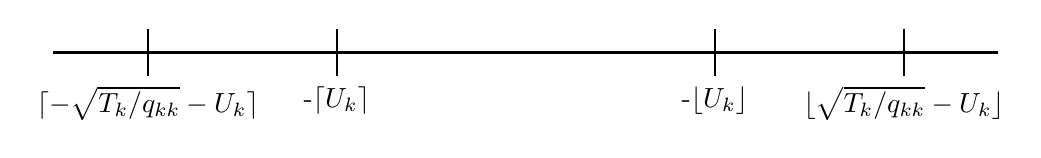
\begin{tikzpicture}[scale=6]
\draw[thick] (0.8,0.05)--(0.8,-0.05) node[anchor=north] {$\lfloor \sqrt{T_k/q_{kk}} - U_k \rfloor$};
\draw[thick] (-0.8,0.05)--(-0.8,-0.05) node[anchor=north]{$\lceil -\sqrt{T_k/q_{kk}} - U_k \rceil$};
\draw[thick] (0.4,0.05)--(0.4,-0.05) node[anchor=north] {-$\lfloor U_k \rfloor$};
\draw[thick] (-0.4,0.05)--(-0.4,-0.05) node[anchor=north]{-$\lceil U_k \rceil$};
\draw[thick] (-1,0)--(1,0);
\end{tikzpicture}
\end{center}

As stated above, 
\[\lceil -\sqrt{T_k/q_{kk}} - U_k \rceil= LB_k \leq y_k \leq UB_k = \lfloor \sqrt{T_k/q_{kk}} - U_k \rfloor.\]
In our old implementation for non-translated lattices, we set each $y_k = LB_k$ and increased each term until we reached the zero (centre) vector. Here since the centre vector is non-zero, we instead set each $y_k = -\lceil U_k \rceil$ and increase each $y_k$ successively until $y_k > \lfloor \sqrt{T_k/q_{kk}} - U_k \rfloor$. This is equivalent to the above computation and generates only half of the vectors, assuming symmetry. This symmetry can only be applied if the centre vector is defined over $\mathbb{Z}$, otherwise we must compute all vectors. To do (we can also break symmetry and compute all vectors in the $\mathbb{Z}$ case), we also set $y_k = \lceil U_k \rceil - 1$ and successively decrease this term until $y_k <\lceil -\sqrt{T_k/q_{kk}} - U_k \rceil$.

Of course, in this refinement, we want to avoid computing $\sqrt{T_k/q_{kk}}$, and so instead of verifying whether $y_k > \lfloor \sqrt{T_k/q_{kk}} - U_k \rfloor$ or $y_k <\lceil -\sqrt{T_k/q_{kk}} - U_k \rceil$, we compute $q_{kk}(y_k + U_k)^2$ in each case and verify whether
\[q_{kk}(y_k + U_k)^2 \leq C - \sum_{i = k+1}^m q_{ii}(y_i + U_i)^2\]
holds. In the first round, if this does not hold and if $y_k < -\lfloor U_k \rfloor$, we continue to iterate $y_k = y_k + 1$, otherwise we simply iterate $y_k = y_k + 1$. Once this equivalence does not hold and $y_k \geq -\lfloor U_k \rfloor$, we stop this loop. We then reset $y_k = \lceil U_k \rceil - 1$ and search in the other direction, by successively subtracting $1$ if 
\[q_{kk}(y_k + U_k)^2 \leq C - \sum_{i = k+1}^m q_{ii}(y_i + U_i)^2\]
holds. We stop searching in this direction only once this equivalence does not hold.  

%--------------------------------------------------------------------------------------------------------------------------------------------%

\endinput

Let
\[g(t) = g_{i1}(t)\cdots g_{im}(t)\]
be the decomposition of $g(t)$ into irreducible polynomials $g_{ij}(t) \in \mathbb{Q}_{p_i}[t]$. The prime ideals in $K$ dividing $p_i$ are in one-to-one correspondence with $g_{i1}(t), \dots, g_{im}(t)$, and in particular, $\deg(g_{ij}(t)) = e_{ij}f_{ij}$. 



Any text after an \endinput is ignored.
You could put scraps here or things in progress.


